%% example for producing articles in MVA format using LaTeX.
%% written by Takeshi MASUDA, Electrotechnical Laboratory, Japan in May 1996.
%% modified by KAGESAWA Masataka, OKAZAKI Shin'ichro, YASUMOTO Mamoru.
%% last modified by Masaki Onishi, AIST, in Nov 2012.
%% use at your own risk.
% * <zzzheng@udel.edu> 2016-12-10T12:01:36.988Z:
%https://preview.overleaf.com/public/dxwcpvfymsxf/images/a5c5f2fd09095ef57c95468d54ed0f9aeaa6d7af.jpeg
% ^.
\documentclass{article}
\usepackage{spconf_2,amsmath,graphicx}
\usepackage{algorithm}  
\usepackage{color}  
%\usepackage[hypcap]{caption}  
\usepackage{multirow} 
\usepackage{comment}
\graphicspath{ {images/} }

\title{Biomedical Document Parsing and Extraction via Image Analysis and Structured Data Analysis}
\name{Scott Sorensen, Abhishek Kolagunda, Zhenzhu Zheng, Xiangyin Jiang, Pengyuan Li, Hagit Shatkay, Chandra Kambhamettu\thanks{This work has been funded by NIH grant BLAH}}
\address{Computer and Information Sciences Department \\University of Delaware
\\ Newark, DE, USA}


\begin{document}
\maketitle


\begin{abstract}
Parsing PDF files and extracting not only text but information contained in figures is critical to data mining and other tasks. Widely varying formats and underlying document structure make the process of extracting these elements challenging. Existing approaches can miss important elements or hyper-fragment figures. We approach this problem using a combination of visual analysis and by parsing the structured document. We combine these extraction techniques with caption matching approach using a metric voting scheme. Experimental results show robust performance for figure extraction and caption matching on challenging biomedical literature.
\end{abstract}

\section{Introduction}
Figures and captions are key sources of information in academic literature. Extraction of these components is a necessary step for creating a snapshot of the publication, which is critical for data mining and tasks such as information retrieval and semantically parsing documents or generating document summaries. Existing tools are able to detect figures, however the nature of biomedical literature means there are many failure cases.

Many challenges stem from the complex nature of figures and the diverse publication formats. Figures not only include a diverse set of image, but also graphs, and plots. Furthermore these components may be raster or vector images, and a single figure can contain many vector elements. This makes successfully detecting all kinds of figures a difficult task. Not all of the images in a document are Figures either, as many publications contain logos and banners. Existing tools for extracting figures and other components of a document mis-classify regions of the document that contain text heavy figures as text, or mis-classify  text if it is near graphical elements or contains mathematical symbols.  

In this paper, we propose a document parsing scheme by solving two problems: figure extraction and caption matching. For figure extraction, our strategy is to exploit image processing as well as freely available PDF tools. While existing tools are already able to handle certain types of figures, the visual approach introduced here aims to provide a complementary role, allowing for undetected figures to be extracted. 

We propose a figure/text separation approach (visual-analysis component) based on the three visual measurements: solidity, size and density. This allows each pixel to be categorized as either background, figure, or text. Finally, we merge the results of the proposed visual-analysis component and an existing PDF tool.

For caption matching, we propose a metric voting scheme based on similarity proximity.Being different from \cite{clark2016pdffigures} which made certain assumptions about caption locations, we intend to cover more general rules about the potential locations of captions. 

The proposed framework is shown in Fig. \ref{fig:framework} and consists of three components. These components are a pdf-Parser, a Visual-Analysis module and a Caption-Matching module. 
\begin{itemize}
	\item[(1)] The \textbf{\textit{pdf-Parser}} component aims at locating text regions of PDF, and also extract text information which  facilitate caption extraction and matching later on. 
	\item[(2)]The \textbf{\textit{Visual-Analysis}} component aims to extract figures using image processing techniques. 
	\item[(3)]The \textbf{\textit{Caption-Matching}} component assigns blocks of text to the corresponding figures based on the voting scheme. In this stage, output of the other modules is utilized to estimate if a text block is a captions and match it to the appropriate figure. 
\end{itemize}

These modules allow our system to better extract figures, and accurately match them to captions. This code will be made available to the public upon publication, allowing the community to utilize these techniques for datamining and other applications. The rest of this paper is organized as follows FILL THIS IN WITH APPROPRIATE SECTIONS ETC.

\begin{figure*}[tb] % figure
\centering
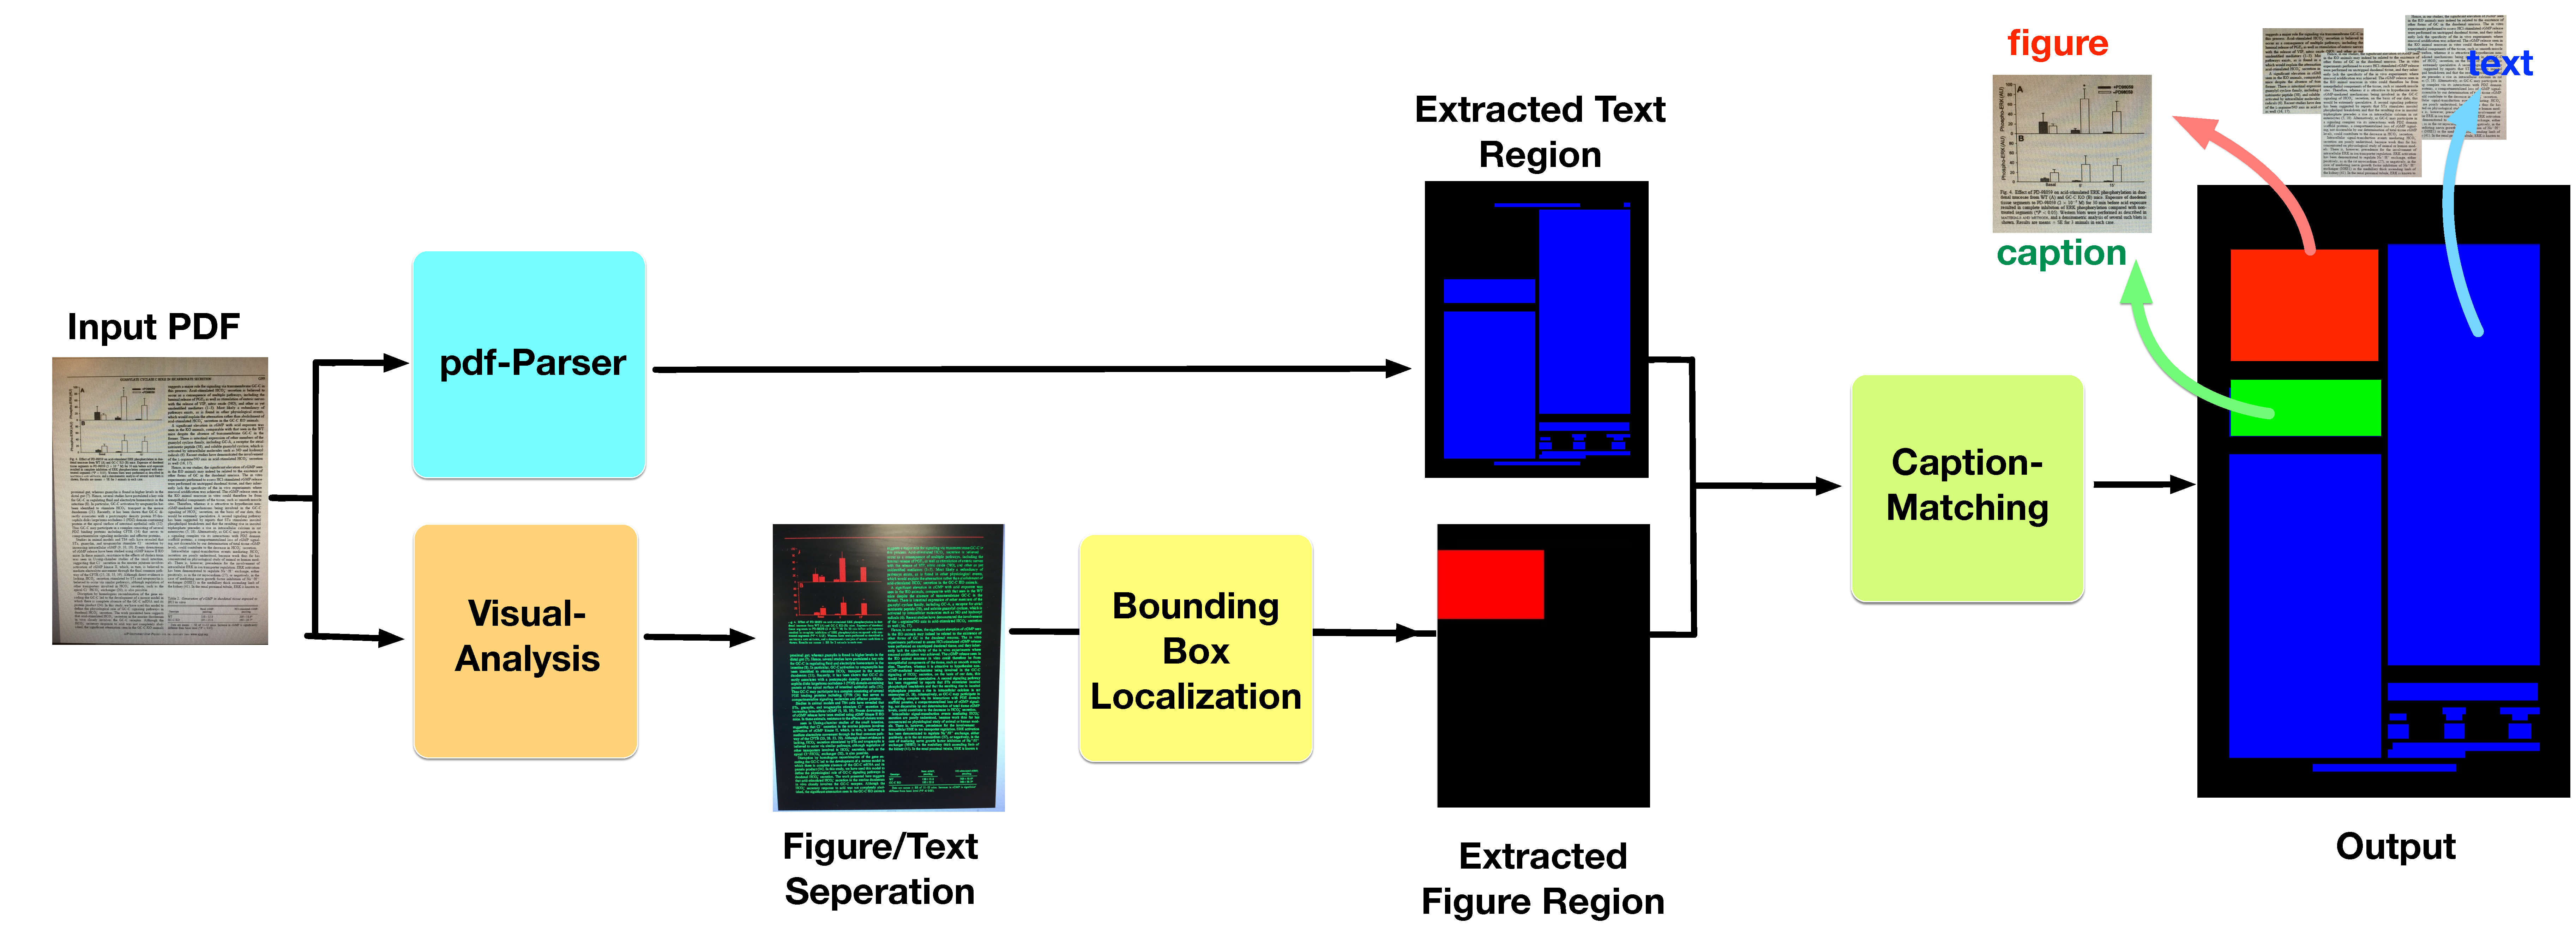
\includegraphics[width=150mm]{Framework} 
\caption{
Overview}
\label{fig:framework}
\end{figure*}

\section{Related Work}
There are a number of tools and applications that have aimed at extracting different page elements from PDF files. Many of these 
tools have targeted figure extraction \cite{ray2015automatic, choudhury2015automated}. There are limited work handle these together. 


Captions are also useful information too. However, some PDF tools, such as PDFBox \cite{pdfbox2014processing} or Poppler \cite{poppler}, leave the problem of caption association unsolved.
Thus, parsing PDF document has became a topic of recent research interest
 \cite{lopez2011automatic,praczyk2013automatic,choudhury2013figure,clark2015looking,clark2016pdffigures}.
Our work is mostly similar with \cite{clark2016pdffigures}.The difference is that
we render the PDF into an image and tend to solve the problem in visual analysis view.
Also, \cite{clark2016pdffigures} mainly focus on parsing PDF files in the Computer Science domain. 
In this study, we aim to build a PDF parsing tool for general publications, not limited to specific domains. Some research has been conducted in the past few years.
\cite{lopez2011automatic} propose an automatic system to extract figures and captions based on the specification of PDF layouts. However, large reasoning is required and it is not likely to generalize well on other documents with a different format style. In this paper, we solve the problem with the deployment of a visual analysis component, and then incorporate with an existing PDF tool in a unified framework. 

\section{PDFMiner}
Existing PDF tools can be utilized to extract figure and text. In this paper, we use pdfminer \cite{shinyama2010pdfminer} to get and analyze layout structure of a PDF file. 
One property is that PDFMiner is able to exact locations of figures. Though there might be missing figure
Also, PDFMiner allows us to obtain the exact location of text in a page, which will facilitate to locating key words in the caption matching module. Further, PDFMiner is able to extract text in blocks, making it easy to extract captions as a whole (see Sec.\ref{sec:CaptionMatching}). 

The pfdminer sometimes fails to detect figures in the pdf. Hence we developed a visual analysis module that takes as input a pdf document and classifies regions of the page as figure or text. ImageMagick is used to convert a pdf to an image. A threshold is applied on an image $I$ to identify foreground pixels (content). The threshold is set such that any pixel that is not $White$ is identified as a foreground pixel. We attempt to classify each foreground pixel as a being a part of a figure or text. Three different metrics, Solidity, Size and Density, are computed for each pixel and used to differentiate between text and figure. An illustration is shown in Fig.
To detect figures and text, we define rules using these metrics. We make the following observations in a page of the pdf documents.

\section{Image-Analysis}
The image-analysis component intends to pickup some figures undetected by pdfminer. We observe that there are some "blank regions" - either classified as text or figure - according to pdfminer layout output. While experimental results show that text extraction has been handled quite well, we consider those "blank regions" as potential figures. To further confirm the "blank region" is figure or not, statistical measurement is applied on the corresponding location in the original PDF page.
In this implementation, we first convert the PDF page into gray-scale image with pixel value ranging from 0 to 1.  


\section{Purification}



\section{Caption Matching}
\label{sec:CaptionMatching}
Existing attempts to extract figures and their matching captions have made a number of assumptions that do not hold for many types of biomedical documents [CITE]. Captions in these documents can occur above or below, or  to either side of figures. They are not always centered, they are not the same width or height, and are not necessarily adjacent. To facilitate accurate figure-caption matching we have implemented a metric voting scheme. The main idea behind the voting scheme is that there are lots of different criteria that imply a specific caption should match to a specific figure, but there are exceptions and failure cases to any one of these potential criteria. We have used a number of different proximity metrics to measure the likelihood that a  caption matches a given figure. Using a voting scheme where different proximity metrics vote on figure-caption matches allows robust matching because individual metrics may get erroneous results, but as an aggregate they perform well. The only assumption made about the position of the caption and figure we make is that they are on the same page, and this assumption is very rarely violated.

For each page we identify figures using extracted figure areas and the visual analysis methods outlined above. Captions are found by searching for key words in text. While it is tempting to just search the first word in a given text box for key words like `Figure', or `Fig', the nature of the PDF format means that some files contain abnormal formatting, and overlapping bounding boxes, and what appears to be the first word or portion of text is not always parsed that way. We search the entire body of text for the substring `fig', to find potential captions. Once we have each figure and each candidate caption we calculate all pairwise metrics and then each metric votes on which caption it matches to.

We have implemented the following metrics for proximity.

\renewcommand{\labelitemi}{\textendash}
\begin{itemize}
\item \textbf{Projection Overlap} measures the maximum amount of overlap between the bounding boxes when they are projected onto the axes. The rationale behind this metric is that figures and captions tend to be in line with the caption below or adjacent to a figure, so matches are likely to overlap in one dimension or another.
\item  \textbf{Edge Distance} measures the minimum edge to edge distance between the bounding boxes for both the figure and the caption. This distance is measured in 1D if there is any overlap in the projection of each bounding box to the axes, or 2D Euclidian distance between closest corner points if there is no overlap. The reasoning behind this metric is that figures and captions tend to be adjacent to each other, and therefore their edges are typically adjacent.
\item  \textbf{Centroid Distance} measures the minimum Manhattan distance between the centers of the figure and caption bounding box. This metric is motivated by the observation that figures and captions are typically both spatially close and inline with each other.
\item  \textbf{Minimum Bounding Box Area} measures the mimimum area of a bounding box that contains the entire figure and caption area. This metric leverages the fact that matching figures and captions are not typically located at different ends of the page.

\end{itemize}
Each metric computes the caption it finds to be the most likely match for a given figure, and then votes are tallied across all the metrics. The candidate caption with the most votes is said to be the match.


\section{Experiments}
\begin{figure*}[t] % figure
\centering
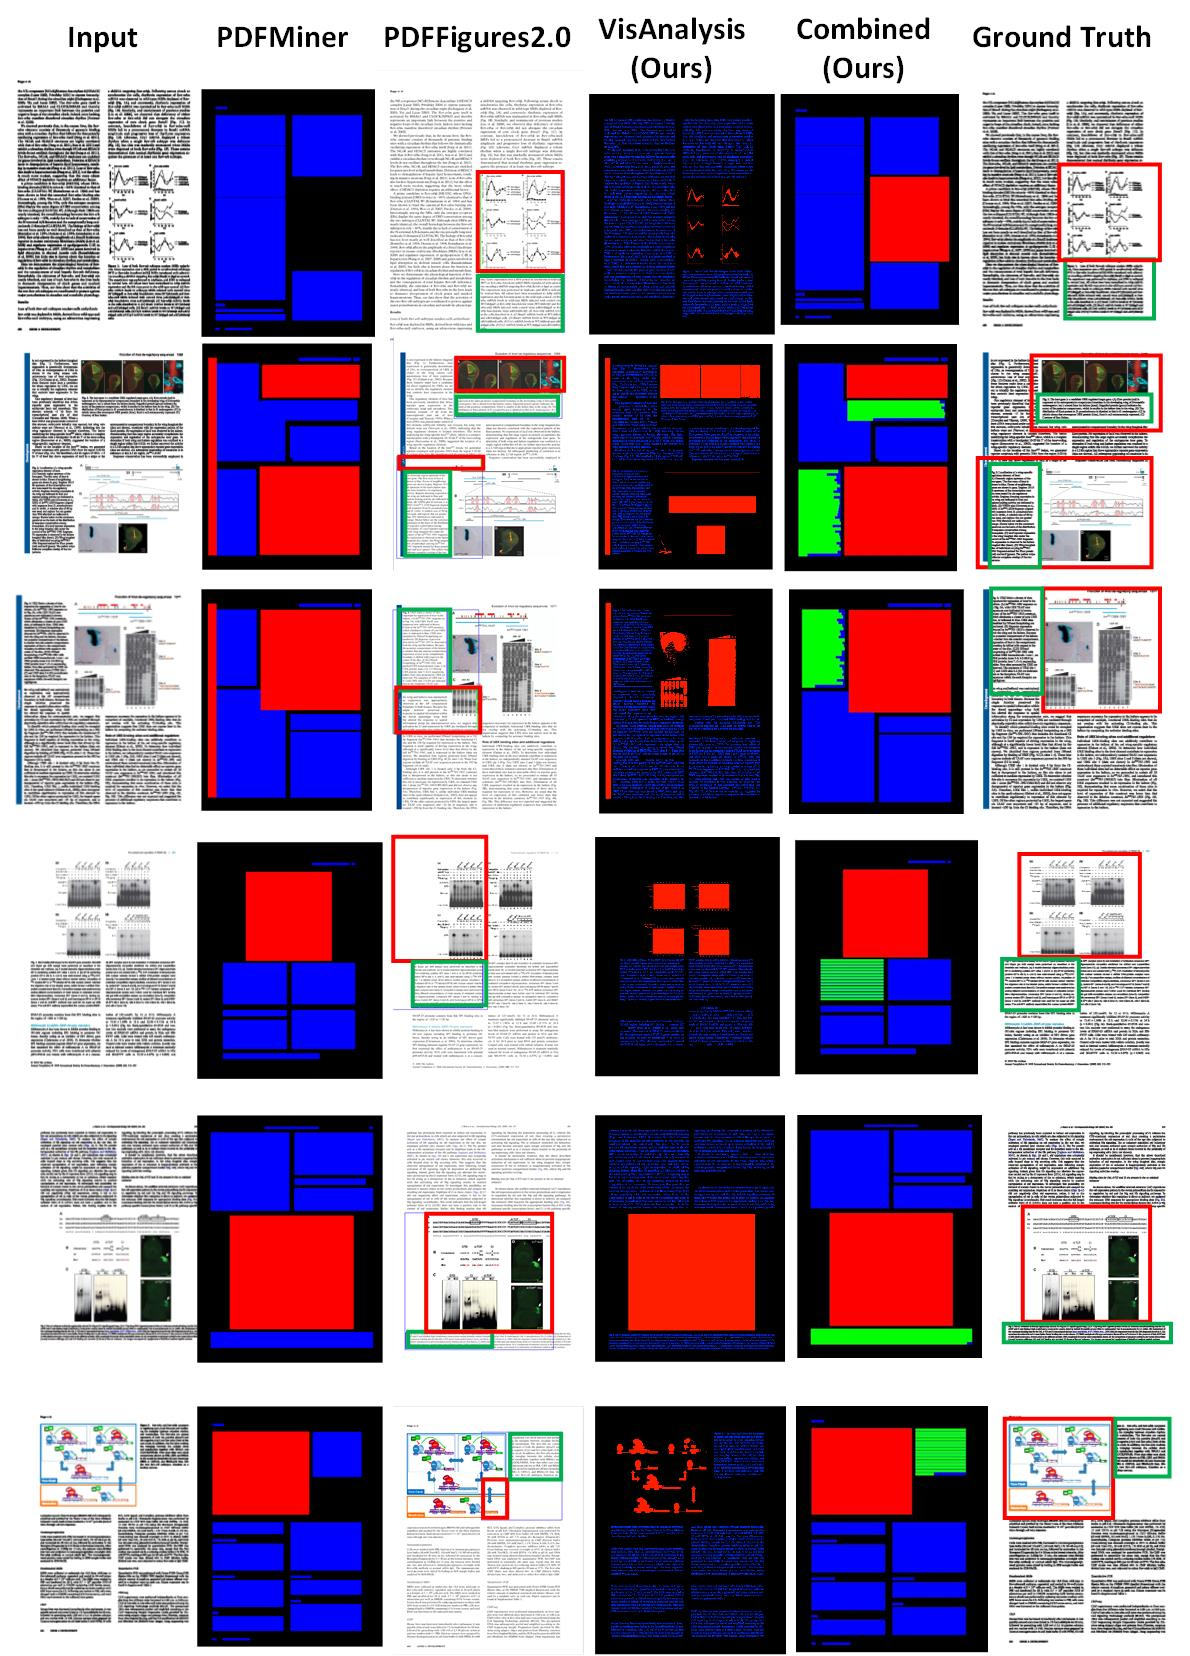
\includegraphics[width=160mm]{Results_part.jpg} 
\caption{
Results. Red indicates figures, green indicates captions, blue indicates texts. Better viewed in color.}
\label{fig:results}
\end{figure*}

In this experiment, We tested the proposed framework on 10 selected documents from popular biomedical journals. There are totally 72 figures, which includes images of DNA sequences, line plot, bar plot and graph. 
We follow similar evaluation procedure as object detection. 
A figure is judged by comparing the bounding boxes detected by the algorithm against the ground truth using the overlap score criterion, similar to Intersection over Union (IoU) for object detection. We consider the output as correct if the overlap score exceeds 0.95, otherwise as incorrect. Caption are scored using the same criterion for the extraction part, and being assigning to the correct figure as well. 
we set a high overlap score here since missing a little part of the figure would not be helpful in the real-world applications. 

For the figure detection task, We compare the proposed framework with one of the existing PDF tools (pdfminer), our proposed visual analysis component, and pdffigures2.0 \cite{clark2016pdffigures}. 

For the caption detection and matching task, we only report results of \cite{clark2016pdffigures} and ours, since general PDF tools (e.g. pdfminer) nor the visual analysis method can do the job. 

Table \ref{tab:pr_fig} and \ref{tab:pr_cap} shows that our framework achieve high recall {\color{blue}X}, than a single component of pdfminer or Visual Analysis. It shows pdfminer has the lowest performance. Results show that the pdfminer incline to fail at figures with DNA sequence and plots. One possible reason is that DNA sequence is somehow visually similar with text, and thus unlikely detected as figures. Also, the special pattern of plots (e.g.line plot, bar plot) diverging from general images brings challenges. Among the three, the proposed framework has the best performance. It can be attributed to the merging results of both pdfminer and VisAnalysis. This is, our proposed VisAnalysis scheme can somehow pick up the left figures which are not detected pdfminer. 
We obtain precision as high as 1, that means no false positives are claimed. This is due to the pruning procedure that unlikely regions (e.g. bar, logos) have been filtered out.

Fig. \ref{fig:results} shows comparison results. While PDFFigures 2.0 \cite{clark2016pdffigures} was originally tested on computer science publications, experiments show that it does not perform well on biomedical publications in more diverse format style. Thus, \cite{clark2016pdffigures} does not perform well, such as figures are not in standard double columns, non-rectangle figure layout, and with compound figures. Also, it inclines to miss caption part when figure located at the bottom (see row 5 in Fig \ref{fig:results}).

For the caption detection task, we get relatively high performance. 
This is because the detection of caption is based on the discovery of figure. Thus, accurate localization of figures and the robust voting scheme would facilitate for caption matching. 

Fig.\ref{fig:results} shows results of figure detection and caption matching. 
The first and second rows show PDF pages with line plot figures which PDF tool failed to detected. VisAnalysis component has successfully capture the pixels for the figure. And the rectangle region is successfully detected by the combined framework (ours). 
The third and fourth rows show PDF pages actually without figures. However, logo and banners have been identified as figures according to VisAnalysis and PDF Tool. With the filtering scheme, the combined framework is able to filter out regions that are unlikely to be figures.

%% TABLE %%
\begin{table}[t]
  \caption{Precision and recall on figure extraction.}
  \begin{center}
    \begin{tabular}{c | c c c}
      \hline
      \hline
      \makebox[10mm]{Method} & \makebox[10mm]{Precision} & 
      \makebox[10mm]{Recall} & \makebox[10mm]{F1}\\
      \hline
      pdfMiner & 0.6667 & 0.7945   & 0.7250 \\
      PDFFigures2.0 \cite{clark2016pdffigures} & 0.9672 & 0.8194 & 0.887 \\
      VisAnalysis (Ours)& 0.6947   & 0.9041 & 0.7857 \\
      Combined (Ours)& \textbf{1.000}   & \textbf{0.9589}   & \textbf{0.9790} \\
      \hline
      \hline
    \end{tabular}
    \label{tab:pr_fig}
  \end{center}
\end{table}


\begin{table}[h]
  \caption{Precision and recall on caption extraction.}
  \begin{center}
    \begin{tabular}{c | c c c}
      \hline
      \hline
      \makebox[10mm]{Method} & \makebox[10mm]{Precision} & 
      \makebox[10mm]{Recall} & \makebox[10mm]{F1}\\
      \hline
       PDFFigures2.0 \cite{clark2016pdffigures} & \textbf{1.000}  &0.8611 & 0.9254 \\
       Combined (Ours) & \textbf{1.000}  & \textbf{0.8889} & \textbf{0.9412} \\
      \hline
      \hline
    \end{tabular}
    \label{tab:pr_cap}
  \end{center}
\end{table}

\section{Conclusion}
In this paper we have presented a framework for extracting figures and their matching captions from PDF documents. The work has targetted 

%%%%%%%%%
% new bibliography
\bibliographystyle{IEEEbib}
\bibliography{reference}


\end{document}
